\begin{frame}{Similarity score and Entropy}
	
	
%	\begin{columns}
%		\column{0.5\textwidth}
%			\begin{figure}
%				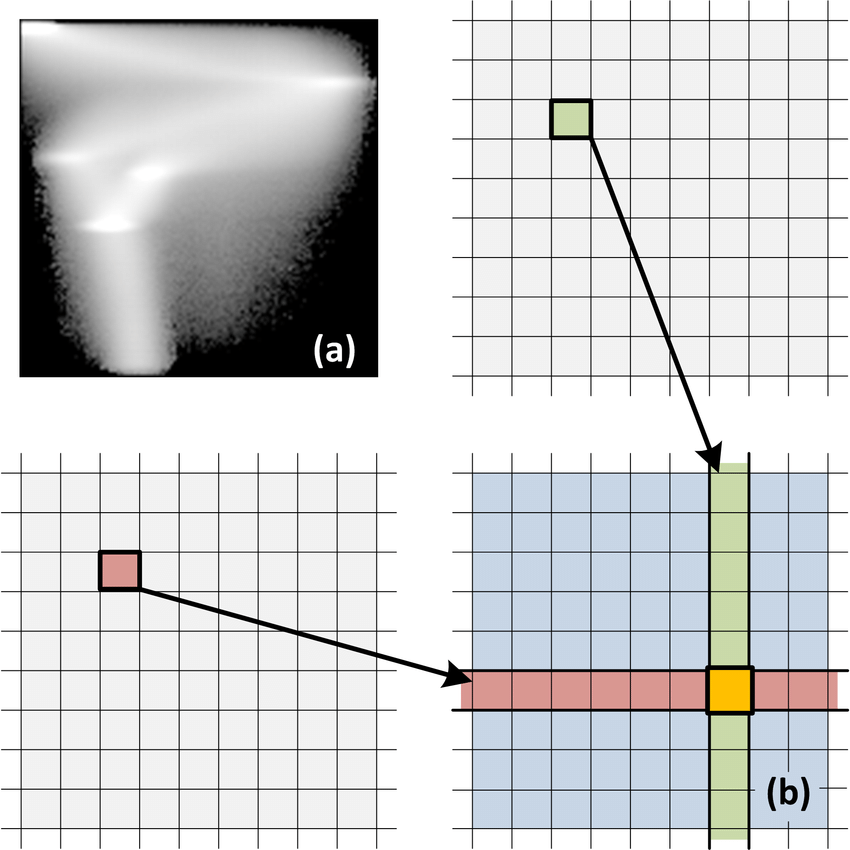
\includegraphics[width=0.5\textwidth]{joint_histogram}
%				\caption{\tiny Joint histogram calculation, from Groots \emph{et al.}, \emph{Practical Examples of GPU Computing Optimization Principles} (2010)}
%				\label{fig:joint_histogram}
%			\end{figure}
%		\column{0.5\textwidth}
%			Joint histogram: matrix $M$
%			$m_{i,j}$ = number of pixels at same position having values i (1st image) and j (second image)
%		Similar images $\implies$ fills diagonal
		
%		For each cell, calculate
%	\end{columns}
	
	$\mathnormal{C_{similarity}}$ relies on histograms and entropy calculation. 
	
	A formula for entropy $H(X)$:
	\begin{equation}
		\mathnormal{H\left(X\right)=-\sum _{i=1}^{n}{P}_{i} * log_{2}\left({P}_{i}\right)}
	\end{equation}
	with:
	\begin{itemize}
		\item $\mathnormal{n}$ the number of different values for pixels,
		\item $\mathnormal{P_{i}}$ probablity distribution of the value $i$ (values of histogram)
	\end{itemize}
	
	Sum of products : feasible with matrix-matrix multiplication
	
	$\implies$ Doable by Tensor cores.
	

\end{frame}